\documentclass[a4paper,12pt]{article}


\usepackage{amsmath}
\usepackage{authblk}
\usepackage{booktabs}
\usepackage[margin=1in]{geometry}
\usepackage{mathtools}
\usepackage{dsfont}
\usepackage{bm}
\usepackage{mdframed}
\usepackage{amsthm}
\usepackage{xfrac}
\usepackage{tikz}
\usetikzlibrary{arrows}

\newcommand{\p}[1]{\mathds{P}\left\{#1 \right\}}
\newcommand{\pp}[1]{\mathds{P}_{\phi} \left\{#1 \right\}}
\newcommand{\pth}[1]{\mathds{P}_{\vartheta} \left\{#1 \right\}}
\newcommand{\pph}[1]{\mathds{P}_{\phi_h} \left\{#1 \right\}}
\newcommand{\ppt}[1]{\mathds{P}_{\phi_t} \left\{#1 \right\}}
\newcommand{\e}[1]{\mathds{E}[#1]}

\newcommand{\fca}{\phi_{\text{case}}}
\newcommand{\fco}{\phi_{\text{control}}}

%opening
\title{A Likelihood Approach to Somatic Mid-Size Indel Calling Under Alignment and Typing Uncertainty}
\author{Louis Dijkstra}

\begin{document}

\maketitle


\section{Introduction} \label{sec:intro}

% Somatic mutations
% Matched tumor/control samples 
% Tumor sample contains healthy diploid cells as well (impurity)
% Next-generation sequencing: Alignment uncertainty & Typing uncertainty

% Variant allele frequency estimation 
% Genotyping (special case)

% Likelihood construction
% Likelihood ratio test
% Multiple testing

\subsection{Notation} \label{sec:notation}

\section{Methods} \label{sec:methods}
The methods presented in this section are based on the following assumptions: 
\begin{itemize}
 \item[\textit{(A1)}]{Reads are independent with respect to their alignment uncertainties, i.e., the probability that a read originates from a certain position on the genome does not depend on the alignment probability of another read;}
 \item[\textit{(A2)}]{The read generating process does not favor particular chromosomes, i.e., a read is a priori equally likely to stem from any chromosome present in the sample;}
 \item[\textit{(A3)}]{The alignment quality of a read is not (heavily) influenced by the presence/absence of the variant allele.}
\end{itemize}
We will throughout the text note explicitly when these assumptions come into play. Note that assumption \textit{(A2)} entails that a variant-allele-affected chromosome is equally likely to bring forth a read as a chromosome that does not harbor the allele. 

\subsection{Variant allele frequency (\textsc{VAF}) estimation}
Let $R = \{R_1, R_2, \dots, R_m \}$ be the set of reads. Every read $R_i \in R$ is associated with two events:
\begin{enumerate}
 \item $A_i^R$ -- the read $R_i$ stems from the locus/region of interest, and 
 \item $V_i^R$ -- the read $R_i$ stems from a variant-allele-affected chromosome, 
\end{enumerate}
where the superscript $R$ refers to the read's sample (this notation becomes useful when we start to reason about several read samples simultaneously, see Section XXX).  
The probability $\p{A_i^R}$ is commonly provided by the aligner. The conditional probability $\p{V_i^R \mid A_i^R}$, i.e., the chance that $i$-th read comes from a variant-allele-affected chromosome given that the read stems from the locus of interest, can often be estimated, see Section XXX. Throughout the rest of the paper, we will use $a_i^R$ and $v_i^R$ as a shorthand notation for $\p{A_i^R}$ and $\p{V_i^R \mid A_i^R}$. For the rest of this section, these quantities are assumed to be known for every read.   

Let us in addition define for every subset $S \subset \{1,\dots,m\}$ the event $A_S^R$ that only the reads $R_i$ with $i \in S$ originate from the locus of interest, while all other reads in $R$ do not. Since reads are independent w.r.t. to their alignment probabilities \textit{(A1)}, its probability is given by
\begin{equation}
 \p{A_S^R} =  \prod_{i \in S} \p{A_i^R} \prod_{j \not \in S} \left(1 - \p{A_j^R} \right) = \prod_{i \in S} a_i^R \prod_{j \not \in S} \left(1 - a_j^R \right). 
 \label{eq:subset}
\end{equation}

Let $\phi \in \Phi \subset [0,1]$ be the variant allele frequency\footnote{The possible values of the \textsc{vaf} $\phi$ in $\Phi$ can often be restricted to a finite set, e.g., for diploid organisms $\Phi = \{0, \sfrac{1}{2}, 1\}$, since either none, only one or two chromosomes can harbor the variant allele. In some cases, it can be rather unclear how to pick $\Phi$; for tumor samples the number of distinct haplotypes are often unknown. Working with the unit interval $\Phi = [0,1]$ can then be a pragmatic solution. We will return to the choice of $\Phi$ in more extent later in the paper.} (\textsc{vaf}), i.e., the fraction of haplotypes that carry the variant allele. In this section, we set out to estimate this quantity using maximum likelihood given the read data in $R$ and the alignment and typing uncertainties as expressed by the probabilities $\left\{(a_i^R, v_i^R)\right\}_{i=1}^m$. 

The likelihood fucntion $\mathcal{L} : \Phi \rightarrow [0,1]$ returns the probability of observing data $R$ in the case of a \textsc{vaf} equal to $\phi$, i.e., 
$\mathcal{L}(\phi) = \pp{R}$. (We use $\pp{\cdot}$ to explicitly denote when the probability measure depends on the parameter $\phi$). 
Since only the reads in $R$ that truely stem from the locus of interest can provide information about $\phi$, the likelihood function can be written as
\begin{equation}
  \mathcal{L}(\phi) = \sum_{S \subset \{1,\dots,m\}} \pp{A_S^R} \pp{R \mid A_S^R},
\end{equation}
where $\pp{R \mid A_S^R}$ is the probability to observe $R$ given that only the reads $R_i$ with $i \in S$ stem from the locus and the other reads do not. By assumption $\emph{(A3)}$ the probability $\pp{A_S^R} = \p{A_S^R}$ (reads stemming from a variant-allele-affected chromosome are equally likely to be aligned correctly as other reads) and is, therefore, given by eq. (\ref{eq:subset}). 
Since reads are assumed to be independent \emph{(A1)}, one can write 
\begin{equation}
 \pp{R \mid A_S^R} = \prod_{i \in S} \pp{R_i \mid A_i^R} \prod_{j \not \in S} \pp{R_j \mid \overline{A_j^R}}
\end{equation}
where $\pp{R_i \mid A_i^R}$ and $\pp{R_i \mid \overline{A_i^R}i}$ are the probabilities of observing read $R_i$ given that it either stems ($A_i^R$) or does not stem ($\overline{A_i^R}$) from the locus of interest. Let us first derive $\pp{R_i \mid A_i^R}$. Under assumption \emph{(A2)} read $R_i$ stems from a variant-allele-affected chromosome with probability equal to the \textsc{vaf} $\phi$ (and, similarly, does not descend from a chromosome carrying the variant allele with probability $1 - \phi$). Due to typing uncertainties, one commonly only knows whether the read stems from a variant-allele-affected chromosome up to a certain level $v_i^R$. The probability to observe a read $R_i$ given that it stems from the locus of interest is, therefore,
\begin{equation}
  \begin{aligned}
 \pp{R_i \mid A_i^R} & = \phi \cdot \p{V_i^R \mid A_i^R} + (1 - \phi)\left(1 - \p{V_i^R \mid A_i^R} \right) \\ & = \phi \cdot v_i^R + (1 - \phi)\left(1 - v_i^R \right). 
  \end{aligned}
  \label{eq:f}
\end{equation}
The probability $\pp{R_j \mid \overline{A_j^R}} = \p{R_j \mid \overline{A_j^R}}$ does not depend on $\phi$ since the variant allele frequency only tells us something about the reads stemming from the locus of interest. Since the read must stem from somewhere on the genome, the probability of observing this read given that it does not cover our region is equal to $1$.  

Combining these results yields an expression for the likelihood of $\phi \in \Phi$ given the read data $R$ and the alignment and typing uncertainties  $\left\{(a_i^R, v_i^R)\right\}_{i=1}^m$ : 
\begin{equation}
 \mathcal{L}(\phi) = \sum_{S \subset \{1,\dots,m\}} \prod_{i \in S} a_i^R \left[\phi \cdot v_i^R + (1 - \phi)\left(1 - v_i^R \right) \right] \prod_{j \not \in S} \left(1 - a_j^R\right). 
\end{equation}
Computing this likelihood would on first glance requires summing over all possible subsets of reads, which entails exponential runtime in the number of reads. Fortunately, this expression can be rewritten as  
\begin{equation}
  \begin{aligned}
  \mathcal{L}(\phi) & = \prod_{i = 1}^m \left\{a_i^R \left[\phi \cdot v_i^R + (1 - \phi)\left(1 - v_i^R \right)\right] + \left(1 - a_i^R\right) \right\} \\
		    & = \prod_{i = 1}^m \left[\phi \cdot  a_i^R\left(2 v_i^R - 1 \right) + 1 - a_i^R v_i^R \right]
  \end{aligned}
\end{equation}
which is linear in the number of reads. 






\subsubsection{Genotyping: the di- and polyploid case}

$\phi \in \Phi_c = \{0, \sfrac{1}{c}, \sfrac{2}{c}, \dots, 1\}$. 
\begin{equation}
 \widehat{\phi}_c = \text{max} \{ \mathcal{L}_\text{c}(0), \mathcal{L}_\text{c}(\sfrac{1}{c}), \mathcal{L}_\text{c}(\sfrac{2}{c}), \dots, \mathcal{L}_\text{diploid}(1) \}. 
\end{equation}


$\phi \in \Phi_{\text{diploid}} = \{0, \sfrac{1}{2}, 1\}$. 
\begin{equation}
 \mathcal{L}_\text{diploid}(\phi) = \begin{dcases}
				      \prod_{i = 1}^m \left(1 - a_i^R v_i^R\right) & \text{if } \phi = 0, \\ 
				      \prod_{i = 1}^m \left(1 - \frac{a_i^R}{2}\right) & \text{if } \phi = \sfrac{1}{2}, \\ 
				      \prod_{i = 1}^m \left(1 - a_i^R v_i^R - a_i^R\right) & \text{if } \phi = 1. 
                                    \end{dcases}
\end{equation}

\begin{equation}
 \widehat{\phi}_\text{diploid} = \text{max} \{ \mathcal{L}_\text{diploid}(0), \mathcal{L}_\text{diploid}(\sfrac{1}{2}), \mathcal{L}_\text{diploid}(1) \}. 
\end{equation}

\subsubsection{The continuous case}
The previous approach of enumerating all possible values of $\phi$ and computing and comparing their respective likelihoods becomes for obvious reasons infeasible when we allow $\phi$ to vary over the unit interval. 

The loglikelihood function $\ell$ is easily found to be 
\begin{equation}
 \ell(\phi) = \log \mathcal{L}(\phi) \sum_{i = 1}^m \log \left\{\phi \cdot  a_i^R\left(2 v_i^R - 1 \right) + 1 - a_i^R v_i^R \right\}.  
\end{equation}
We find that its second order derivative is
\begin{equation}
 \frac{\partial^2 \ell}{\partial \phi^2} = - \sum_{i = 1}^m \left [ \frac{a_i^R \left(2 v_i^R - 1\right)}{\phi \cdot a_i^R \left(2 v_i^R - 1\right) + 1 - a_i^R v_i^R }\right]^2 < 0
\end{equation}
for all $\phi \in [0,1]$ given that there is at least one read that potentially stems from the locus of interest and provides information on the presence/absence of the variant allele, i.e., $\exists i \in \{1, \dots, m\}$ for which $a_i^R > 0$ and $v_i^R \neq \sfrac{1}{2}$. Therefore, the loglikelihood function is, under this weak condition, a strictly concave function, and therefore possesses one unique global maximum on the unit interval. 




\subsection{Likelihood construction for somatic mutation calling}

Suppose we are presented with two matched data sets of reads, $C = \{C_1, \dots, C_m\}$ and $D = \{D_1, \dots, D_n\}$, where $C$ is the control sample of (presumed) healthy, diploid cells and $D$ is the disease sample: a set of reads that stem from a mixture of tumor and healthy cells. Let $\alpha \in [0,1]$ denote the fraction of chromosomes in this disease-control mixture $D$ that are from healthy cells, commonly referred to as the \emph{level of impurity}. For the moment we assume $\alpha$ to be known. 

In order to assess whether a somatic mutation occured, we need to determine the frequency with which the variant allele occurs in both healthy and tumor cells. We will denote these quantities with, respectively, $\phi_h$ and $\phi_t$ (where the `$h$' reffers to healthy and `$t$' to tumor). In the case that the variant is absent in healthy cells, i.e., $\phi_h = 0$, and present in tumor cells, i.e., $\phi_t > 0$, we speak of a somatic mutation. 

Since healthy cells are diploid, the values $\phi_h$ can take are contained in $\Phi_h = \{0, \sfrac{1}{2}, 1\}$, since either zero, one or two chromosomes can harbor the allele. The frequencies with which the variant can occur among tumor cells are harder to establish. Ideally, one would know the number of distinct haplotypes present in the tumor. Unfortunately, estimates on this number are hard to obtain. We, therefore, choose to vary $\phi_t$ over the unit interval, i.e., $\Phi_t = [0,1]$, thereby avoiding the need to specify this quantity. Although it might be superfluous to treat a discrete quantity such the \textsc{vaf} as a continuous one, we feel that assuming continuity will not heavily undermine the performance of the method presented here.  

More formally, we are interested in estimating the parameter $\vartheta = (\phi_h, \phi_t) \in \Theta$, where 
\begin{equation}
 \Theta = \Phi_h \times \Phi_t = \{(\phi_h, \phi_t) : \phi_h \in \{0, \sfrac{1}{2}, 1\}, \phi_t \in [0,1] \}
\end{equation}
is our parameter space. The likelihood function $\mathcal{L}_{\textsc{sm}} : \Theta \rightarrow [0,1]$ is the probability of observing the case and control data sets given the parameter $\vartheta$, i.e., $\mathcal{L}_{\textsc{sm}} (\phi_h, \phi_t) = \mathds{P}_{\phi_h, \phi_t} \{C , D\}$. Due to the independence of the control and case sample, this probability can be written as  
\begin{equation}
 \mathcal{L}_{\textsc{sm}} (\phi_h, \phi_t) = \mathds{P}_{\phi_h} \{C\} \mathds{P}_{\phi_h, \phi_t} \{D\} 
\end{equation}
where we used the fact that the healthy sample $C$ is not influenced by the tumor \textsc{vaf} $\phi_t$. Note that due to impurity, quantified by $\alpha$, the disease sample $D$ does provide information about the $\textsc{vaf}$ of healthy cells, $\phi_h$. 
The first term $\mathds{P}_{\phi_h} \{C\}$ is identical to the likelihood of $\phi_h$ in the diploid case, see eq. (XXX). Determining $\mathds{P}_{\phi_h, \phi_t} \{D\} $ is slightly more involved, but similar to the derivation of the likelihood function for the \textsc{vaf} in Section XXX. Again, only the reads in $D$ that actually stem from the locus of interest carry information about $\vartheta$, i.e., 
\begin{equation}
 \mathds{P}_{\phi_h, \phi_t} \{D\} = \sum_{S \in \{1,\dots,n\}} \p{A_S^D} \mathds{P}_{\phi_h, \phi_t} \left\{ D \mid A_S^R \right\}
\end{equation}
where we used assumption \emph{(A3)} and $\p{A_S^D}$ is given in eq. (\ref{eq:subset}). Due to the independence of reads \emph{(A1)}, we can write 
\begin{equation}
 \mathds{P}_{\phi_h, \phi_t} \left\{ D \mid A_S^R \right\} = \prod_{i \in S} \mathds{P}_{\phi_h, \phi_t} \left\{D_i \mid A_i^D\right\} \prod_{j \not\in S} \mathds{P}_{\phi_h, \phi_t} \left\{D_j \mid \overline{A_j^D} \right\}
\end{equation}
where $\mathds{P}_{\phi_h, \phi_t} \left\{D_j \mid \overline{A_j^D} \right\}$ is again equal to $1$. Under assumption \emph{(A2)}, the read $R_i$ stems with probability $\alpha$ from a healthy cell and with probability $1 - \alpha$ from a tumor cell. Therefore, 
\begin{equation}
 \mathds{P}_{\phi_h, \phi_t} \left\{D_i \mid A_i^D\right\} = \alpha \mathds{P}_{\phi_h} \left\{D_i \mid A_i^D\right\} + (1 - \alpha) \mathds{P}_{\phi_t} \left\{D_i \mid A_i^D\right\}. 
\end{equation}
The probabilities $\mathds{P}_{\phi_h} \left\{D_i \mid A_i^D\right\}$ and $\mathds{P}_{\phi_t} \left\{D_i \mid A_i^D\right\}$ are given by eq. (\ref{eq:f}). The probability $\mathds{P}_{\phi_h, \phi_t} \{D\} $ is, therefore,  
\begin{equation}
 \begin{aligned}
  \mathds{P}_{\phi_h, \phi_t} \{D\} & = \sum_{S \in \{1,\dots,n\}} \prod_{i \in S} a_i^D \left[ \alpha \mathds{P}_{\phi_h} \left\{D_i \mid A_i^D\right\} + (1 - \alpha) \mathds{P}_{\phi_t} \left\{D_i \mid A_i^D\right\} \right] \prod_{j \not \in S} \left(1 - a_i^D \right) \\
  & = \prod_{i = 1}^n \left\{ a_i^D \left[ \alpha \mathds{P}_{\phi_h} \left\{D_i \mid A_i^D\right\} + (1 - \alpha) \mathds{P}_{\phi_t} \left\{D_i \mid A_i^D\right\} \right] + \left(1 - a_i^D \right) \right\}. 
 \end{aligned}
\end{equation}
Combining these results yields the following expression for the likelihood $\mathcal{L}_\textsc{sm}(\phi_h, \phi_t)$: 
\begin{equation}
 \begin{aligned}
  \mathcal{L}_\textsc{sm}(\phi_h, \phi_t) & = \mathds{P}_{\phi_h} \{C\} \mathds{P}_{\phi_h, \phi_t} \{D\}  \\ 
   & =  \prod_{i = 1}^m \left[a_i^C \phi_h \left(2 v_i^C - 1 \right) + 1 - a_i^C v_i^C \right] \times \\ 
  & \qquad  \prod_{i = 1}^n \left[ a_i^D \left(\alpha \phi_h + (1 - \alpha) \phi_t \right) \left(2 v_i^D - 1 \right)  + 1 - a_i^D v_i^D \right]. 
 \end{aligned}
\end{equation}


\begin{equation}
 \mathcal{L}_{\textsc{sm}} (\phi_h, \phi_t) = \begin{dcases}
	\prod_{i = 1}^m \left( 1 - a_i^C v_i^C \right) \times \prod_{i = 1}^n \left[ a_i^D \phi_t (1 - \alpha)\left(2v_i^2 - 1\right) + 1 - a_i^D v_i^D \right] & \text{if }\phi_h = 0 \\ 
	\prod_{i = 1}^m \left( 1 - \frac{a_i^C}{2} \right) \times \prod_{i = 1}^n \left[ a_i^D \left(\phi_t (1 - \alpha) + \frac{\alpha}{2} \right) \left(2v_i^D - 1 \right) + 1 - a_i^D v_i^D \right] & \text{if }\phi_h = \sfrac{1}{2} \\ 
	\prod_{i = 1}^m \left( 1 - a_i^C v_i^C - a_i^C \right) \times \prod_{i = 1}^n \left[ a_i^D \left(\phi_t (1 - \alpha) + \alpha \right) \left(2v_i^D - 1 \right) + 1 - a_i^D v_i^D \right] & \text{if }\phi_h = 1 \\ 
  \end{dcases}
\end{equation}


$$
  \frac{\partial^2 \ell (\vartheta)}{\partial \phi_t^2} = - \sum_{i = 1}^n \left[ \frac{a_i^D (1 - \alpha) \left(2 v_i^D - 1 \right)}{a_i^D \left( \phi_t (1 - \alpha) + \alpha \phi_h \right) \left(2 v_i^D - 1 \right) + 1 - a_i^D v_i^D} \right]^2 \leq 0
$$
Strictly concave iff $\alpha < 1$ and $\exists i \in \{1,\dots,n\}$ for which $a_i^D > 0$ and $v_i^D \neq \sfrac{1}{2}$. 



\subsection{Testing for somatic mutations: A Likelihood ratio test for non-nested models}

\begin{equation}
 \Theta_{\textsc{sm}} = \{(\phi_h, \phi_t) : \phi_h = 0, \phi_t \in (0,1]\}. 
\end{equation}
$\Theta_0 = \Theta \setminus \Theta_{\textsc{sm}}$. 


$$
H_0 : \vartheta \in \Theta_0 \qquad \text{versus} \qquad H_a : \vartheta \in \Theta_{\textsc{sm}}
$$

\begin{figure}
  \centering
 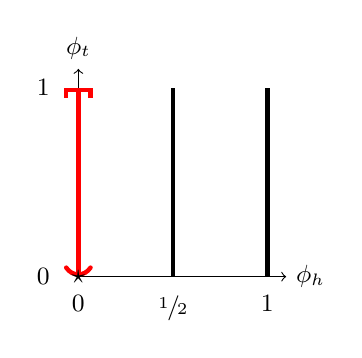
\begin{tikzpicture}[scale = 1.2]
  \draw[->] (0,0) -- (0,2.2) node [above] {\small $\phi_t$} ; 
  \draw[->] (0,0) -- (2.2,0)  node [right] {\small $\phi_h$} ; 
  
  %\draw[ultra thick] node[below] {\small $0$} (0,0) -- (0,2) ;
  \draw[ultra thick] (1,0) -- (1,2) ; 
  \draw[ultra thick] (2,0) -- (2,2) ; 
  
  \draw node[below] at (0,-0.1) {\small $0$} ; 
  \draw node[below] at (1,-0.1) {\small $\sfrac{1}{2}$} ; 
  \draw node[below] at (2,-0.1) {\small $1$} ; 
  \draw node[left] at (-0.2,0) {\small $0$} ; 
  \draw node[left] at (-0.2,2) {\small $1$} ; 
  \draw[[-), ultra thick, red] (0,2) -- (0,0);
  \draw node at (0,0) {$\star$} ; 
 \end{tikzpicture}
 \caption{The parameter space $\Theta$. The red interval $(0,1]$ at $\phi_h = 0$ is $\Theta_\textsc{sm}$ and denotes the cases where a somatic mutation occured. The parameters related to the situation where no mutation occured are depicted with black, including the origin $(0,0)$ which is for clarity shown here with a $\star$. }
\end{figure}


\end{document}